The main idea behind this project was to use the \textit{Pandaboard} - an embedded development board - to output information on an external device, in this case a LED bar with 40 LED's. The goal was to create the drivers and to be able to use it universally. We wanted to create the possibility to write different applications for this system, without changing anything on the driver level of the \textit{Pandaboard}. 
Examples for so called \textit{User-space} application are measuring the quality of a connected WLAN, measuring the signal strength of a WLAN and also to output the \textit{Load} - CPU usage - of the \textit{Pandaboard}.

\section{Pandaboard}

\begin{figure}[H]
   \centering
   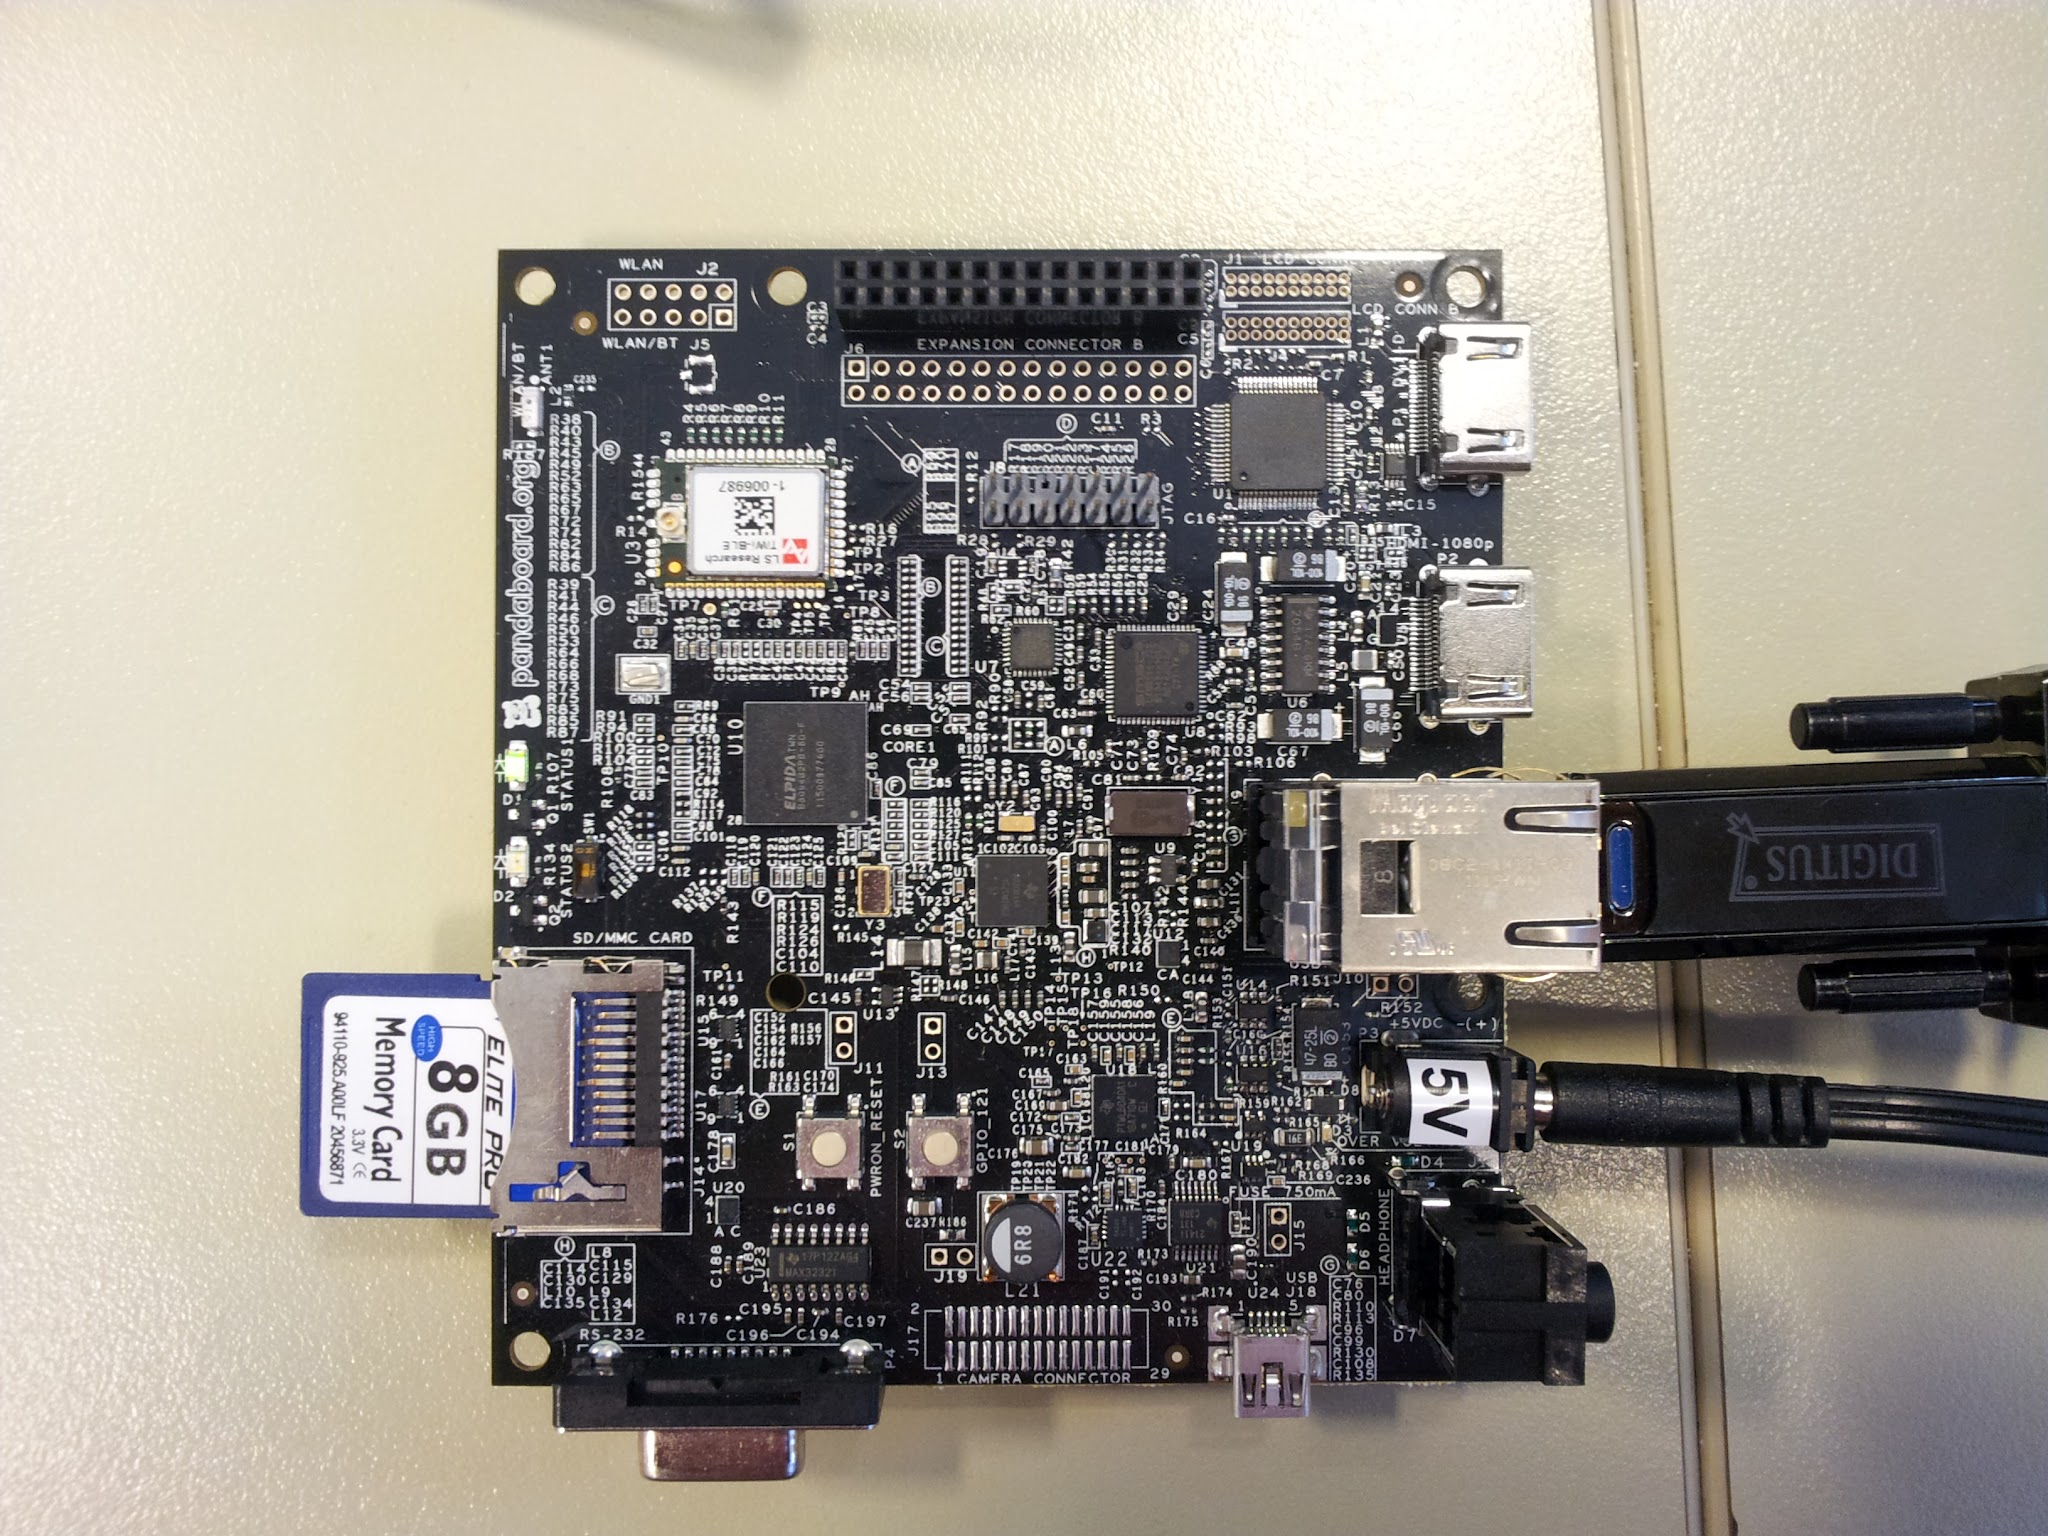
\includegraphics[width=0.8\textwidth]{img/Pandaboard_Alone.jpg}%
   \caption{Pandaboard with installed SD card}
   \label{fig:pandaBoard_Alone}%
\end{figure}

\section{LED-Bar}
\begin{figure}[H]
   \centering
   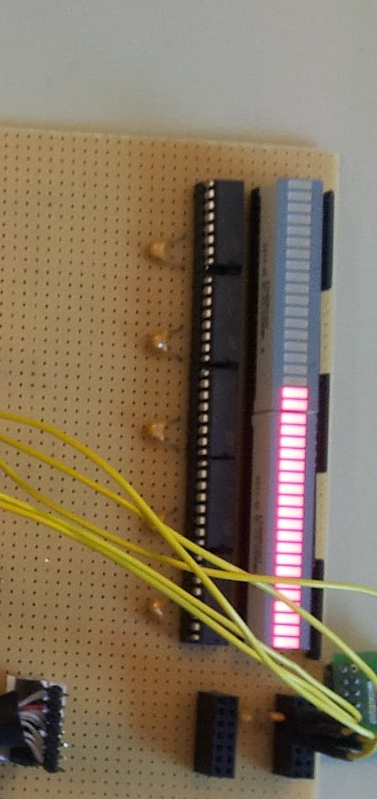
\includegraphics[width=0.3\textwidth]{img/LED-Bar.png}%
   \caption{LED-Bar with 40 LED's and level-shifter.}
   \label{fig:ledBar}%
\end{figure}

\section{Goal to achieve}
\begin{figure}[H]
   \centering
   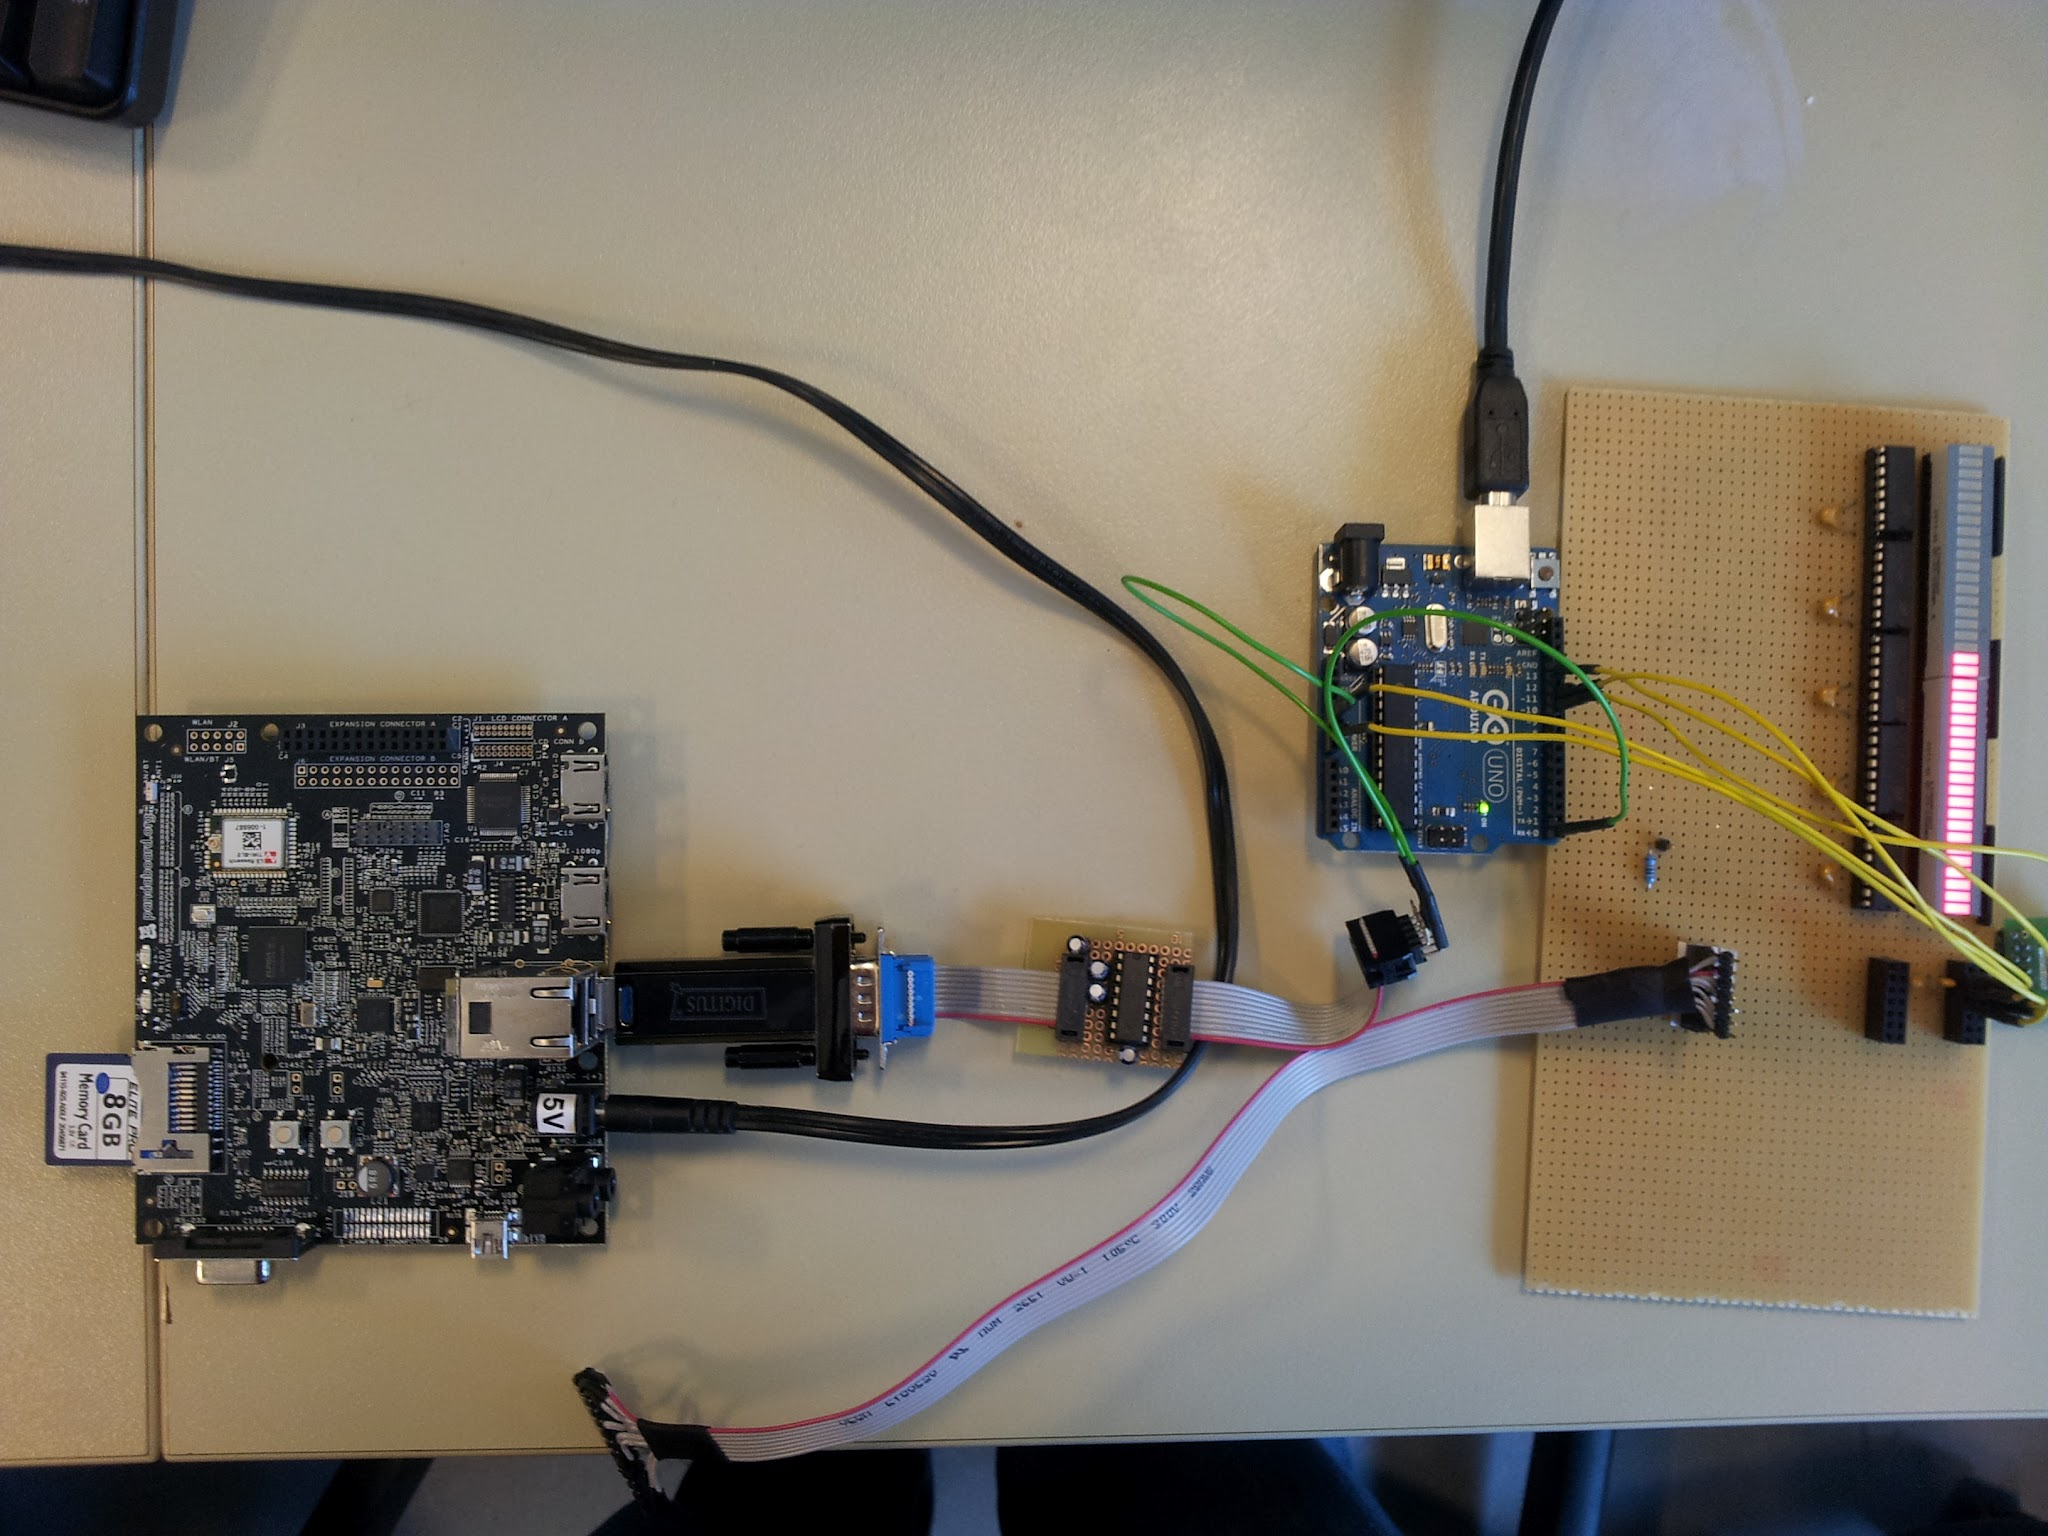
\includegraphics[width=0.8\textwidth]{img/Panda_and_LED_Bar.jpg}%
   \caption{Powering the LED-bar with the Pandaboard and a microcontroller}
   \label{fig:completeProject}%
\end{figure}